\chapter{Note de cadrage}

\section{Contexte}

\subsection{Good Food : présentation de l'entreprise}
Good Food est une franchise de restauration créée en 1992, issue de la fusion de quatre entreprises indépendantes. La marque s’est développée progressivement via une logique de réseau et de franchise, avec une croissance soutenue depuis les années 1990.

Aujourd’hui, l’enseigne compte :
\begin{itemize}
    \item 150 restaurants répartis en France, Belgique et Luxembourg
    \item Environ 1\,000 collaborateurs
    \item Plus de 200 recettes proposées
    \item Environ 1 million de repas livrés par an
    \item 80 \% du chiffre d’affaires réalisé via la vente en ligne
\end{itemize}

Le réseau est composé de nombreux franchisés dont les besoins peuvent varier (menus spécifiques, promotions locales, fournisseurs dédiés, etc.). Cette diversité implique une forte hétérogénéité des pratiques opérationnelles et une nécessité d’offrir une plateforme adaptable, tout en conservant un socle commun pour garantir la cohérence de marque, la qualité de service et l’industrialisation.

\subsection{Organisation interne}
Le siège de Good Food est volontairement réduit, avec environ 30 collaborateurs répartis dans les services suivants :
\begin{itemize}
    \item Comptabilité
    \item Communication et community management
    \item Service informatique restreint composé de 4 personnes, majoritairement orienté support de niveau~1
\end{itemize}

Le développement des solutions informatiques est historiquement sous-traité. Cette organisation a permis d’aller vite, mais a progressivement créé une dépendance aux prestataires, une visibilité limitée sur la qualité du code et une capacité d’évolution contrainte.

Les prestataires actuels sont :
\begin{itemize}
    \item \textbf{PWI} : hébergement de l’infrastructure et supervision
    \item \textbf{WIM} : développement de l’application de commande en ligne et synchronisation avec l’ERP
    \item \textbf{TP System} : déploiement et gestion des terminaux de paiement
    \item \textbf{BNB} : services bancaires et paiements en ligne
\end{itemize}

\subsection{L’application actuelle : limites et problématiques}
L’application de commande en ligne actuellement en production présente de nombreuses faiblesses :
\begin{itemize}
    \item Développement initial en 1998 (Java), refonte en 2005 en ASP.NET (C\#)
    \item Hébergement sur Windows Server 2008 R2, dont le support est arrêté
    \item Code obsolète, peu documenté et difficilement maintenable
    \item Accumulation de correctifs successifs sans vision d’ensemble
    \item Performances insuffisantes et bugs récurrents (codes promotionnels, panier)
    \item Absence totale d’application mobile
    \item Multiples adaptations spécifiques pour les franchisés, non maîtrisées
\end{itemize}

Ce système ne répond plus aux exigences actuelles du marché en termes de performance, d’évolutivité et de maintenabilité. Il constitue également un risque opérationnel majeur, car la vente en ligne représente une part dominante du chiffre d’affaires : toute indisponibilité, lenteur ou régression fonctionnelle a un impact direct sur les revenus, la satisfaction client et l’image de marque.

\section{Objectifs du projet}

Le projet vise la refonte complète de l’application de commande en ligne de Good Food. Cette plateforme représente un enjeu stratégique majeur puisqu’elle génère environ 80 \% du chiffre d’affaires de l’entreprise. L’objectif est d’obtenir une solution moderne, robuste et évolutive, capable de soutenir la croissance du réseau et d’améliorer significativement l’expérience utilisateur.

Les objectifs principaux sont les suivants :
\begin{itemize}
    \item Migrer vers des technologies open source modernes et pérennes afin de réduire les risques de dépendance et d’obsolescence.
    \item Développer une application mobile (iOS/Android) pour répondre aux nouveaux usages (commande rapide, suivi, fidélité, notifications).
    \item Garantir une haute disponibilité du service lors des pics de commandes (déjeuners, soirées, événements, promotions).
    \item Mettre à disposition des franchisés un service dédié pour la gestion de leurs opérations (commandes, préparations, fournisseurs et livraisons).
\end{itemize}

Cette refonte s’accompagne d’une transformation organisationnelle avec la création progressive d’un pôle informatique interne (renforcement des compétences, reprise en main de l’architecture, industrialisation de la livraison et de la qualité).

Le nouveau système devra également :
\begin{itemize}
    \item S’intégrer à l’écosystème existant (ERP Dynamics~365, Sage, systèmes de paiement), via des interfaces maîtrisées.
    \item Conserver l’intégralité des données historiques, avec une migration transparente pour la production.
    \item Respecter les engagements de développement durable (optimisation des ressources, sobriété, traçabilité).
\end{itemize}

\section{Parties prenantes}

Les principales parties prenantes du projet sont :
\begin{itemize}
    \item \textbf{Clients finaux} : utilisateurs web/mobile (commande, paiement, suivi, réclamations).
    \item \textbf{Franchisés} : gestion opérationnelle (menus, promotions, commandes, fournisseurs, livraisons).
    \item \textbf{Direction} : pilotage stratégique, image de marque, continuité d’activité.
    \item \textbf{Comptabilité} : consolidation, rapprochements, flux financiers, intégration Sage / EBICS.
    \item \textbf{Communication} : gestion des retours et réclamations, suivi de la satisfaction.
    \item \textbf{DSI / SI} : architecture cible, sécurité, maintien en condition opérationnelle, gouvernance technique.
    \item \textbf{Prestataires et partenaires} : hébergeur, paiement, TPE, éditeurs (ERP, banque).
\end{itemize}

\section{Équipe projet et rôles}

L’équipe projet est structurée pour couvrir l’architecture, le delivery et l’industrialisation :
\begin{itemize}[leftmargin=0pt,label={},itemsep=0.6em]
  \item \textbf{Product Owner (Gabriel):}\\
  {\small Priorisation, gestion du backlog, validation fonctionnelle, arbitrages.}

  \item \textbf{Scrum Master (Lukas):}\\
  {\small Animation agile, levée des obstacles, amélioration continue.}

  \item \textbf{Développeur Backend (Tous):}\\
  {\small APIs métier, intégrations (ERP, paiement), sécurité, performance.}

  \item \textbf{Développeur Frontend (Tous):}\\
  {\small Web app, accessibilité, performance perçue, UX.}

  \item \textbf{Ingénieur DevOps (Fadi):}\\
  {\small CI/CD, environnements, observabilité, déploiement, fiabilité.}

  \item \textbf{Architecte Cloud (Kenan):}\\
  {\small Conception cible, scalabilité, résilience, gouvernance, coûts.}
\end{itemize}

\section{Périmètre fonctionnel cible (synthèse)}
La solution applicative visée doit couvrir les grands domaines suivants :
\begin{itemize}
    \item Gestion des clients (inscription, compte, historique, réclamations)
    \item Authentification et gestion des accès
    \item Gestion des menus et du catalogue
    \item Commande en ligne (panier)
    \item Paiement (en ligne et intégrations)
    \item Organisation des livraisons (créneaux, suivi)
    \item Réservations
    \item Portail franchisé (promotions, fournisseurs, pilotage opérationnel)
    \item Optionnel : analyse de données / aide à la décision
\end{itemize}

% ----------------------------------------------------------------------

\chapter{Organisation Agile et Méthodologie SCRUM}

\section{Framework SCRUM adapté au projet}

\subsection{Cadre organisationnel}
Le projet adopte le framework SCRUM afin de livrer de la valeur par incréments, tout en conservant la flexibilité nécessaire pour intégrer les retours des franchisés et des équipes internes. Les principes structurants retenus sont :
\begin{itemize}
    \item Sprints de deux semaines permettant des livraisons régulières et mesurables.
    \item Équipe cross-fonctionnelle (développement, UX, DevOps) favorisant l’autonomie et la réduction des dépendances.
    \item Cérémonies planifiées à horaires fixes afin d’installer un rythme et une discipline collective.
\end{itemize}

\subsection{Adaptations au contexte Good Food}
Compte tenu des contraintes (legacy, intégrations externes, migration), des aménagements sont prévus :
\begin{itemize}
    \item Un \textbf{Sprint 0} dédié à la mise en place des environnements, de la CI/CD, des conventions et de l’observabilité.
    \item Des démonstrations régulières incluant un panel de franchisés (retours rapides sur la valeur métier).
    \item Un focus particulier sur la \textbf{migration de données} (stratégie progressive, répétable, sécurisée).
\end{itemize}

\section{Rôles et responsabilités}

\subsection{Product Owner}
Le Product Owner, représentant de Good Food, est chargé de :
\begin{itemize}
    \item Définir et prioriser le Product Backlog
    \item Valider les user stories et leurs critères d’acceptation
    \item Assurer l’interface entre les franchisés, la direction et l’équipe projet
\end{itemize}

\subsection{Scrum Master}
Le Scrum Master a pour mission de :
\begin{itemize}
    \item Animer les cérémonies SCRUM
    \item Lever les obstacles rencontrés par l’équipe
    \item Accompagner l’équipe dans l’adoption des pratiques agiles
    \item Assurer le reporting vers le management
\end{itemize}

\subsection{Équipe de développement}
L’équipe de développement est :
\begin{itemize}
    \item Auto-organisée et pluridisciplinaire
    \item Responsable de la qualité technique et fonctionnelle
    \item En charge de l’estimation et de la réalisation des user stories
\end{itemize}

\section{Cérémonies SCRUM}

\subsection{Sprint Planning}
Cette réunion, organisée en début de sprint, définit l’objectif du sprint (Sprint Goal), sélectionne les user stories prioritaires et détaille les tâches techniques nécessaires.

\subsection{Daily Scrum}
Réunion quotidienne de 15 minutes destinée à synchroniser l’équipe, exposer l’avancement et remonter les blocages le plus tôt possible.

\subsection{Sprint Review}
Présentation des fonctionnalités terminées, démonstration et recueil des retours des parties prenantes. Les feedbacks alimentent directement l’ajustement du Product Backlog.

\subsection{Sprint Retrospective}
Analyse du sprint écoulé et identification des axes d’amélioration. Un plan d’action concret est défini pour le sprint suivant.

\section{Artefacts SCRUM}

\subsection{Product Backlog}
Le Product Backlog regroupe l’ensemble des user stories priorisées. Chaque user story est définie avec des critères d’acceptation, incluant des aspects de performance, sécurité et UX lorsque nécessaire.

\subsection{Sprint Backlog}
Le Sprint Backlog contient le périmètre du sprint et les tâches techniques associées. Il est maintenu à jour quotidiennement.

\subsection{Increment}
L’incrément correspond à une version potentiellement livrable, testée, documentée et conforme à la Definition of Done.

% ----------------------------------------------------------------------

\chapter{Indicateurs de suivi et pilotage}

\section{Indicateurs de performance technique}
Les indicateurs suivants permettent d’objectiver la performance et la fiabilité :
\begin{itemize}
    \item Temps de réponse des API (objectif et suivi par percentile)
    \item Disponibilité de la plateforme (SLA/SLO)
    \item Nombre de bugs critiques en production
    \item Couverture de tests automatisés et taux de succès des pipelines
\end{itemize}

\section{Indicateurs de progression du projet}
Le pilotage projet s’appuie sur :
\begin{itemize}
    \item Vélocité de l’équipe et stabilité de la capacité
    \item Burndown chart des sprints et analyse des écarts
    \item Respect des jalons, visibilité sur le reste à faire
    \item Budget consommé vs budget planifié (si applicable)
\end{itemize}

\section{Indicateurs métier}
Pour mesurer la valeur produite, les indicateurs métier suivants sont suivis :
\begin{itemize}
    \item Adoption de la plateforme par les franchisés (onboarding, usage)
    \item Temps moyen de traitement d’une commande (bout en bout)
    \item Satisfaction client (Net Promoter Score, retours, réclamations)
\end{itemize}

% ----------------------------------------------------------------------

\chapter{Planification du projet}

La planification s’articule autour de jalons structurants : mise en place des fondations techniques, livraison progressive des fonctionnalités cœur, intégrations SI, migration de données, puis stabilisation et déploiement généralisé.

\section{Jalons et macro-phases}
\begin{itemize}
    \item \textbf{Phase 0 -- Cadrage \& architecture} : exigences, découpage fonctionnel, architecture cible, risques.
    \item \textbf{Phase 1 -- Fondations} : CI/CD, environnements, sécurité de base, observabilité.
    \item \textbf{Phase 2 -- Fonctionnalités cœur} : compte client, menus, panier, commande, paiement, livraisons.
    \item \textbf{Phase 3 -- Portail franchisés} : opérations, promotions, fournisseurs, pilotage.
    \item \textbf{Phase 4 -- Intégrations SI \& migration} : ERP, Sage/EBICS, paiements, synchronisations.
    \item \textbf{Phase 5 -- Stabilisation \& déploiement} : charge, correction, mise en production progressive.
\end{itemize}

\section{Croquis d'architecture}

\begin{figure}[H]
    \centering
    % Remplace le fichier par ton image (PNG/PDF/SVG->PDF)
    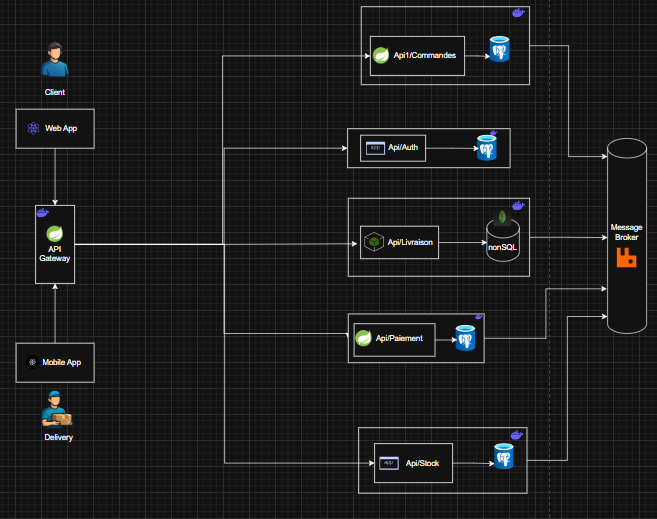
\includegraphics[width=0.95\textwidth]{figures/schema_architecture.png}
    \caption{Croquis de l’architecture cible (vue logique et flux principaux).}
    \label{fig:architecture-sketch}
\end{figure}

\section{Principes d’architecture (à détailler après validation)}
L’architecture cible devra notamment :
\begin{itemize}
    \item Séparer clairement les responsabilités (frontends, API, services métier, intégrations).
    \item Permettre la montée en charge lors des pics de commandes (scalabilité horizontale).
    \item Assurer la résilience (dégradation contrôlée, tolérance aux pannes).
    \item Encadrer les intégrations SI (ERP, paiement) via des interfaces maîtrisées.
    \item Faciliter l’évolutivité (ajout de nouveaux services franchisés, fonctionnalités mobile).
\end{itemize}